% !TEX program = pdflatex
% NOTE: IEEEtran 版本建议使用 pdfLaTeX 编译。
\documentclass[journal]{IEEEtran}
\usepackage{cite}
\usepackage{amsmath}
\usepackage{amssymb}
\usepackage{graphicx}
\IfFileExists{orcidlink.sty}{\usepackage{orcidlink}}{\providecommand{\orcidlink}[1]{}}
\usepackage{tikz-cd}
\usetikzlibrary{arrows.meta,positioning}

\title{Physics-Guided Learned Compensation of Structured Mismatch in Reduced-Reference Cylindrical Aperture 3-D mmW Imaging}
%\title{ReMiC-Net: A Reference-Surface-Aware Mismatch Compensation Network for Reduced-Reference Cylindrical Aperture 3-D Imaging}
\author{Yun Su\orcidlink{0009-0008-5831-9344}, Weixian Tan\orcidlink{0000-0001-9071-9470} \IEEEmembership{Member, IEEE}, Yifan Dong\orcidlink{0000-0002-3155-6437}, Wei Xu\orcidlink{0000-0002-8045-8817} \IEEEmembership{Member, IEEE}, Pingping Huang\orcidlink{0000-0001-7720-1183} \IEEEmembership{Member, IEEE}
}

\begin{document}
\maketitle

\begin{abstract}
Near-field cylindrical aperture radar imaging is an important technique for high-resolution three-dimensional reconstruction in security screening, nondestructive testing, and short-range sensing. However, accurate cylindrical aperture reconstruction requires spatially varying spherical-wave compensation, while fast reference-surface-based algorithms may introduce structured approximation mismatch when the number of reference cylindrical surfaces is aggressively reduced. In this paper, we propose a physics-guided learned compensation framework for reduced-reference cylindrical aperture 3-D imaging. The proposed method retains a reduced-reference cylindrical imaging operator as a low-complexity physical backbone and introduces ReMiC-Net, a reference-surface-aware mismatch compensation network for residual correction and structural restoration. Instead of directly regressing the final image, ReMiC-Net learns the residual between the coarse reduced-reference reconstruction and the target reflectivity, while explicitly using reference-surface-aware geometric metadata, including shell assignment, nearest-reference deviation, valid field-of-view mask, and support prior. A dual-branch architecture with FiLM-style modulation is adopted to inject geometry-aware conditioning into volumetric feature extraction. In addition, an auxiliary support prediction head is introduced to improve extended-target structural preservation. Simulated and experimental results demonstrate that the proposed method substantially improves reconstruction quality, support continuity, and speed--quality trade-off while maintaining a runtime close to the reduced-reference physical backbone. The proposed framework provides an efficient and interpretable learning-assisted solution for compensating structured model mismatch in fast cylindrical aperture 3-D imaging.
\end{abstract}

\begin{IEEEkeywords}
Cylindrical aperture imaging, millimeter-wave radar imaging, physics-guided reconstruction, reference-surface-aware learning, structured mismatch compensation.
\end{IEEEkeywords}

\section{Introduction}
Near-field millimeter-wave and microwave three-dimensional (3-D) imaging has attracted increasing attention in security screening, nondestructive testing, through-wall sensing, and biomedical inspection. Owing to the penetration capability of millimeter-wave signals through common nonmetallic materials and their nonionizing nature, active near-field radar imaging systems can provide high-resolution volumetric information of concealed or weakly visible targets. In these applications, both image quality and reconstruction speed are critical, since the imaging system is often required to reconstruct complex 3-D scenes within a limited acquisition and processing time.

Among various near-field imaging configurations, cylindrical aperture imaging is particularly attractive because it provides wide angular observation and is suitable for full-view 3-D reconstruction of human-scale or object-scale targets. However, cylindrical aperture imaging is also substantially more challenging than planar aperture imaging. Under near-field conditions, the spherical wavefront, free-space propagation loss, nonlinear range history, nonuniform wavenumber-domain sampling, and space-variant point spread function must be properly handled. As a result, the imaging operator cannot be simply represented as a global convolution, and standard fast Fourier transform (FFT)-based algorithms developed for planar apertures cannot be directly applied without additional approximations or coordinate transformations \cite{Fortuny-Guasch_Lopez-Sanchez_2001,Tan_Hong_Wang_Wu_2011,Gao_Deng_Qin_Wang_Li_2018,Wang_Yao_Song_Wang_Sun_2024}.

Backprojection (BP) and matched-filtering-based methods can accurately compensate the spherical-wave propagation path for each voxel, and are therefore commonly regarded as high-fidelity reconstruction approaches. Nevertheless, their voxel-wise coherent summation leads to high computational cost, which restricts their use in real-time 3-D imaging. To improve efficiency, a variety of frequency-domain and wavenumber-domain algorithms have been developed for near-field cylindrical and MIMO imaging. For example, nonplanar measurements can be backpropagated to a planar aperture before applying 3-D range migration \cite{Fortuny-Guasch_Lopez-Sanchez_2001}; spherical wave decomposition, circular convolution, and nonuniform FFT can be exploited for efficient MIMO cylindrical holographic imaging \cite{Gao_Deng_Qin_Wang_Li_2018}; and mixed-domain formulations have been proposed to address space-variant spectral characteristics in more complicated near-field MIMO-SAR configurations \cite{Wang_Yao_Song_Wang_Sun_2024}. These methods have significantly advanced fast 3-D near-field imaging, but they still rely on carefully designed analytical approximations and often exhibit a trade-off between computational efficiency and reconstruction fidelity.

Another important class of fast cylindrical aperture imaging methods is based on reference cylindrical surfaces. The basic idea is to divide the imaging region into cylindrical surfaces with different radii and construct matched filters with respect to selected reference surfaces. By reusing the matched-filtering functions associated with these reference surfaces, the repeated computation of spatially varying focusing kernels can be reduced. Tan et al. developed a spherical-wave 3-D imaging algorithm for cylindrical scanning geometries that explicitly considers wavefront curvature and free-space propagation loss \cite{Tan_Hong_Wang_Wu_2011}. More recently, a high-precision millimeter-wave cylindrical aperture holographic imaging algorithm was proposed, where the imaging region is divided into cylindrical surfaces of different radii, reference cylindrical surfaces are selected according to imaging accuracy and phase-error control, and the complexity of repeated matched-filter computation is reduced \cite{Tan}. This reference-surface strategy provides an efficient and physically interpretable backbone for cylindrical aperture imaging.

Despite its efficiency, reference-surface-based imaging naturally introduces approximation errors when the number of reference surfaces is aggressively reduced. A dense reference-surface library improves focusing accuracy but increases computational cost, whereas a reduced-reference implementation is fast but no longer perfectly matched to the true radial position of every voxel. The resulting error is not random noise; it is a structured, geometry-dependent mismatch governed by the assigned reference surface, radial deviation from that surface, angular observation geometry, and valid field-of-view support. This structured mismatch becomes particularly harmful for extended targets, where boundary continuity, support integrity, and thin structures are more important than isolated peak localization.

Deep learning provides a promising way to compensate such model-induced reconstruction errors. Recent studies in computational electromagnetic imaging have shown that purely data-driven networks may suffer from limited interpretability and generalization, while physics-embedded learning can combine analytical imaging operators with trainable neural networks to improve both efficiency and reconstruction quality \cite{Guo_Huang_Li_Zhang_Eldar_2023}. In near-field 3-D radar imaging, Manisali et al. proposed a two-stage physics-based learned reconstruction framework, where an adjoint physical operator first maps radar measurements to the image domain and a 3-D U-Net then refines the intermediate reconstruction for extended targets \cite{Manisali_Oral_Oktem_2024}. This demonstrates the effectiveness of using a physics-based warm start followed by a deep volumetric network. Related learning-based 3-D SAR and millimeter-wave imaging methods, such as RMIST-Net, further show that embedding analytical operators into neural reconstruction can improve computational efficiency \cite{Wang_Wei_Liang_Zeng_Wang_Shi_Zhang_2022}. However, most existing learning-based radar imaging methods focus on sparse reconstruction, compressive sensing, MIMO array configurations, or generic image-domain refinement. They do not explicitly address the structured mismatch induced by reduced-reference cylindrical aperture imaging.

Model mismatch has also been recognized as a key issue in learning-based 3-D radar reconstruction. For instance, MAda-Net shows that a fixed observation model cannot accurately represent spatially varying observation models in TomoSAR, and that such model inconsistency can cause nonnegligible imaging errors that cannot be fully eliminated by network parameter optimization alone \cite{Wang_Liu_Zhu_Liu_Ding_Zeng_2023}. This observation is closely related to reduced-reference cylindrical imaging: using a small number of reference surfaces is equivalent to forcing a spatially varying cylindrical imaging process to be represented by a limited set of approximate reference models. Therefore, the network should not be treated as a generic post-processing module. Instead, it should be explicitly informed of the reference-surface assignment and the local severity of the approximation error.

In addition, extended-target reconstruction requires more than voxel-wise intensity correction. Recent studies in deep-learning-based TomoSAR reconstruction have shown that spatial features such as edges, regular shapes, and structural continuity can provide useful constraints for 3-D reconstruction, especially when the target scene contains prominent spatial structures \cite{Zeng_Zhan_Ren_Ma_Liu_Shi_Wei_Wang_Zhang_2025}. For reduced-reference cylindrical aperture imaging, extended targets are also the most challenging cases, because reference-surface mismatch may lead to support fragmentation, boundary deformation, and shape distortion. Therefore, a structure-aware compensation strategy is needed to recover not only the intensity distribution but also the target support.

Motivated by these observations, this paper proposes a physics-guided learned compensation framework for structured mismatch in reduced-reference cylindrical aperture 3-D imaging. The proposed method, termed \emph{ReMiC-Net}, is a Reference-Surface-Aware Mismatch Compensation Network for Reduced-Reference Cylindrical Aperture 3-D Imaging. Instead of replacing the analytical imaging operator, ReMiC-Net retains a reduced-reference cylindrical aperture imaging operator as a fast physical backbone. The coarse reconstruction obtained from this backbone is then refined by a residual compensation network conditioned on reference-surface-aware geometric metadata, including shell assignment, nearest-reference deviation, valid field-of-view mask, and support prior. In addition, an auxiliary support prediction head is introduced to improve extended-target structural preservation, including support continuity, boundary integrity, and thin-structure recovery.

The main contributions of this paper are summarized as follows.

\begin{itemize}
    \item We formulate the approximation error of reduced-reference cylindrical aperture imaging as a structured, geometry-dependent mismatch rather than generic image degradation. This formulation provides a problem-driven perspective for learning-assisted fast cylindrical aperture 3-D imaging.

    \item We propose ReMiC-Net, a reference-surface-aware residual compensation network that explicitly uses reference-surface metadata to guide mismatch correction. The network is designed to compensate the reduced-reference approximation error while preserving the low-complexity advantage of the physical backbone.

    \item We design a reference-surface-aware geometry conditioning strategy to guide residual mismatch compensation. The network explicitly uses shell assignment, nearest-reference deviation, valid field-of-view information, and support prior, allowing the compensation behavior to adapt to the local severity of reduced-reference approximation error.

    \item We incorporate an auxiliary support prediction task to improve extended-target structure preservation. The support supervision encourages the network to recover continuous target regions, thin structures, and boundaries that are easily distorted by reduced-reference approximation.

    \item We conduct systematic simulations and experimental evaluations, including point-target validation, extended-target reconstruction, ablation studies, support-structure analysis, runtime comparison, robustness tests, and measured-data validation. The results demonstrate that the proposed method can significantly improve reconstruction quality while maintaining a runtime close to the reduced-reference physical backbone.
\end{itemize}

The remainder of this paper is organized as follows. Section~II introduces the mathematical background of cylindrical aperture 3-D imaging and reduced-reference approximation. Section~III presents the proposed ReMiC-Net framework, including the reference-surface-aware input representation, network architecture, residual compensation strategy, and support-aware loss design. Section~IV reports simulated and experimental results. Section~V concludes this paper and discusses future work.

\section{Mathematical Background}
\label{sec:math_background}

This section formulates the cylindrical aperture near-field imaging model and clarifies the source of the structured mismatch considered in this work. The exact reference-surface selections used for \emph{ref3}, \emph{ref5}, \emph{ref7}, and \emph{ref9} are reported in the experimental section, while this section focuses on the general forward model and the reduced-reference approximation mechanism.

\subsection{Cylindrical Aperture Imaging Geometry}
\label{subsec:geometry}

Consider a monostatic cylindrical aperture imaging system, where a transmit/receive antenna samples the scattered field on a cylindrical surface. The antenna position is denoted as
\begin{equation}
\mathbf{r}'(\phi',z')=
\left[\rho_0\cos\phi',\ \rho_0\sin\phi',\ z'\right]^T,
\label{eq:antenna_position}
\end{equation}
where \(\rho_0\) is the radius of the cylindrical scan, \(\phi'\) is the azimuth sampling angle, and \(z'\) is the elevation position. A voxel in the imaging domain is represented in cylindrical coordinates as
\begin{equation}
\mathbf{r}(\rho,\phi,z)=
\left[\rho\cos\phi,\ \rho\sin\phi,\ z\right]^T,
\label{eq:voxel_position}
\end{equation}
where \(\rho\), \(\phi\), and \(z\) denote the radial, azimuthal, and elevation coordinates, respectively. The propagation distance between the antenna and the voxel is then
\begin{equation}
R(\rho,\phi,z;\phi',z')=
\sqrt{\rho_0^2+\rho^2-2\rho_0\rho\cos(\phi-\phi')+(z-z')^2}.
\label{eq:range}
\end{equation}
This spherical-wave distance term is the central geometric quantity in cylindrical aperture near-field imaging. It makes the phase history dependent on the voxel position and prevents the cylindrical case from being reduced to a simple space-invariant Cartesian convolution.

Fig.~\ref{fig:cylindrical_geometry} shows a schematic illustration of the cylindrical scanning geometry and the use of multiple reference cylindrical surfaces. The concrete reference radii used in the comparative baselines are listed later in Section~IV.

\begin{figure}[!t]
\centering
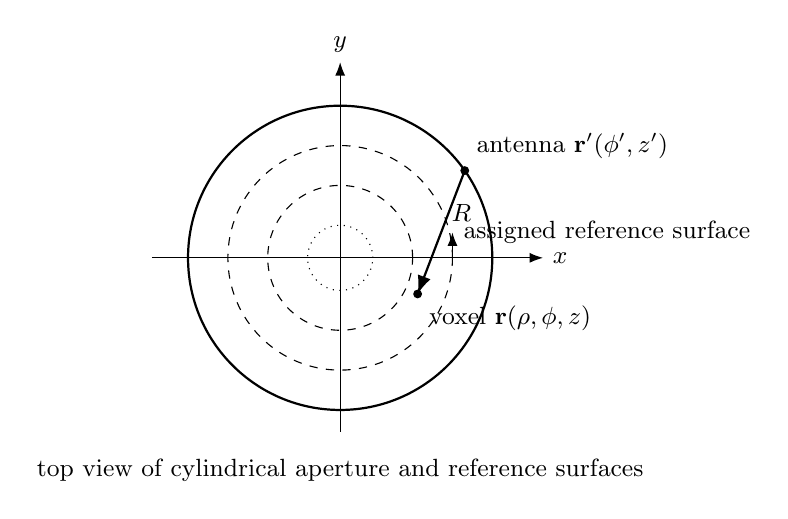
\begin{tikzpicture}[scale=0.92, >=Latex]
    % coordinate axes
    \draw[->] (-2.6,0) -- (2.8,0) node[right] {\small $x$};
    \draw[->] (0,-2.4) -- (0,2.7) node[above] {\small $y$};

    % reference surfaces top view
    \draw[thick] (0,0) circle (2.1);
    \draw[dashed] (0,0) circle (1.55);
    \draw[dashed] (0,0) circle (1.00);
    \draw[dotted] (0,0) circle (0.45);

    % antenna position
    \coordinate (ant) at ({2.1*cos(35)},{2.1*sin(35)});
    \filldraw[black] (ant) circle (1.5pt);
    \node[above right=1pt of ant] {\small antenna $\mathbf{r}'(\phi',z')$};

    % voxel
    \coordinate (vox) at ({1.18*cos(-25)},{1.18*sin(-25)});
    \filldraw[black] (vox) circle (1.5pt);
    \node[below right=1pt of vox] {\small voxel $\mathbf{r}(\rho,\phi,z)$};

    % range arrow
    \draw[->, thick] (ant) -- (vox) node[midway, above right] {\small $R$};

    % reference label
    \draw[->] (1.55,0) -- (1.55,0.35);
    \node[right] at (1.57,0.35) {\small assigned reference surface};
    \node[below] at (0,-2.65) {\small top view of cylindrical aperture and reference surfaces};
\end{tikzpicture}
\caption{Schematic top-view illustration of cylindrical aperture imaging. The antenna samples the scattered field on a cylindrical surface, while the imaging region is represented by voxels with radial coordinate \(\rho\). Reduced-reference imaging uses only a subset of reference cylindrical surfaces to construct approximate matched filters.}
\label{fig:cylindrical_geometry}
\end{figure}

\subsection{Spherical-Wave Forward Model}
\label{subsec:forward_model}

Let \(x(\rho,\phi,z)\) denote the complex-valued 3-D reflectivity distribution of the scene. For a point scatterer, the measured response at the frequency wavenumber \(k=2\pi f/c\) can be expressed as
\begin{equation}
 y_p(k,\phi',z')=
 x(\rho,\phi,z)\frac{\exp[-j2kR(\rho,\phi,z;\phi',z')]}{R^2(\rho,\phi,z;\phi',z')},
\label{eq:point_model_full}
\end{equation}
where the exponential term represents the two-way spherical-wave phase history and \(R^{-2}\) models the free-space propagation loss. In calibrated or amplitude-compensated processing, the amplitude factor may be removed or absorbed into a weighting term, yielding the phase-dominant model
\begin{equation}
 y_p(k,\phi',z')=
 x(\rho,\phi,z)\exp[-j2kR(\rho,\phi,z;\phi',z')].
\label{eq:point_model_phase}
\end{equation}

For an extended target, the received echo is the coherent superposition of all voxel contributions:
\begin{equation}
 y(k,\phi',z')=
 \iiint_{V} x(\rho,\phi,z)
 \exp[-j2kR(\rho,\phi,z;\phi',z')]\, dV
 + n(k,\phi',z'),
\label{eq:continuous_forward}
\end{equation}
where \(V\) is the imaging volume and \(n(k,\phi',z')\) denotes measurement noise and modeling error. This model follows the linearized scattering assumption commonly adopted in holographic microwave and SAR-type imaging; multiple scattering within the object is not modeled.

After discretization, the forward model is written as
\begin{equation}
\mathbf{y}=\mathbf{A}\mathbf{x}+\mathbf{n},
\label{eq:discrete_forward}
\end{equation}
where \(\mathbf{y}\in\mathbb{C}^{M}\) is the measurement vector, \(\mathbf{x}\in\mathbb{C}^{N}\) is the discretized 3-D reflectivity vector, and \(\mathbf{A}\in\mathbb{C}^{M\times N}\) is the cylindrical near-field forward operator. The \((m,n)\)-th element of \(\mathbf{A}\) can be expressed as
\begin{equation}
 A_{m,n}=w_{m,n}\exp[-j2k_m R(\mathbf{r}_n;\phi'_m,z'_m)],
\label{eq:system_matrix}
\end{equation}
where \(w_{m,n}\) denotes the optional amplitude weighting term. When free-space propagation loss has been compensated or ignored, \(w_{m,n}=1\).

The sampling intervals along frequency, azimuth, and elevation are chosen to satisfy the cylindrical aperture sampling constraints to avoid aliasing; the detailed numerical sampling parameters used in this work are provided in Section~IV rather than repeated here.

\subsection{Matched-Filtering Reconstruction}
\label{subsec:matched_filter}

Given the cylindrical echo \(y(k,\phi',z')\), a spherical-wave matched-filtering or backprojection-type reconstruction can be written as
\begin{equation}
 \tilde{x}(\rho,\phi,z)=
 \int_{z'}\int_{\phi'}\int_{k}
 y_R(k,\phi',z')
 \exp[+j2kR(\rho,\phi,z;\phi',z')]
 k\, dk\, d\phi'\, dz',
\label{eq:matched_filter}
\end{equation}
where \(y_R(k,\phi',z')\) denotes the range-gated or amplitude-compensated echo. Eq.~\eqref{eq:matched_filter} can be interpreted as an adjoint-type operation of the forward model in Eq.~\eqref{eq:discrete_forward}. It coherently compensates the spherical-wave phase history for each candidate voxel.

However, because \(R(\rho,\phi,z;\phi',z')\) is nonlinear and spatially varying, direct evaluation of Eq.~\eqref{eq:matched_filter} over a dense 3-D grid is computationally expensive. This motivates accelerated cylindrical reconstruction methods based on wavenumber-domain processing, range stacking, or reference-surface approximation.

\subsection{Reference-Surface-Based Reconstruction}
\label{subsec:reference_surface}

Reference-surface-based cylindrical reconstruction reduces the repeated computation of spatially varying matched filters by dividing the imaging region into a sequence of cylindrical surfaces. Let the full reference-surface library be denoted by
\begin{equation}
\mathcal{S}_{\mathrm{full}}=
\{\rho_1,\rho_2,\ldots,\rho_L\}.
\label{eq:full_reference_library}
\end{equation}
For each reference radius \(\rho_l\), an approximate matched filter is constructed as
\begin{equation}
 H_l(k,\phi',z';\phi,z)=
 \exp[+j2kR(\rho_l,\phi,z;\phi',z')].
\label{eq:reference_filter}
\end{equation}
A full-reference reconstruction operator can then be abstractly represented as
\begin{equation}
 \mathbf{x}_{\mathrm{full}}=\mathcal{R}_{\mathrm{full}}(\mathbf{y}),
\label{eq:full_reconstruction}
\end{equation}
where \(\mathcal{R}_{\mathrm{full}}\) uses a sufficiently dense reference-surface library to approximate the exact spherical-wave focusing process.

In this paper, the detailed radius selections for \emph{ref3}, \emph{ref5}, \emph{ref7}, and \emph{ref9} are not listed in this background section. They are instead reported in Section~IV, together with the simulation and runtime settings, because those selections are part of the experimental protocol.

\subsection{Reduced-Reference Approximation and Structured Mismatch}
\label{subsec:structured_mismatch}

To obtain a low-complexity physical backbone, only a small subset of the full reference library is used:
\begin{equation}
\mathcal{S}_{Q}=\{\rho_{q_1},\rho_{q_2},\ldots,\rho_{q_Q}\},\quad Q\ll L.
\label{eq:reduced_library}
\end{equation}
For a voxel \(v\) with radial coordinate \(\rho(v)\), its assigned reference radius is defined as
\begin{equation}
 \rho_Q^{\ast}(v)=
 \arg\min_{\rho_q\in\mathcal{S}_{Q}} |\rho(v)-\rho_q|.
\label{eq:assigned_reference}
\end{equation}
The corresponding signed radial deviation is
\begin{equation}
 \delta\rho_Q(v)=\rho(v)-\rho_Q^{\ast}(v).
\label{eq:radial_deviation}
\end{equation}
Using this reduced library, the approximate reconstruction is denoted by
\begin{equation}
 \mathbf{x}_{Q}=\mathcal{R}_{Q}(\mathbf{y}).
\label{eq:reduced_reconstruction}
\end{equation}
In particular, the most aggressive low-complexity backbone used in this work is
\begin{equation}
 \mathbf{x}_{\mathrm{ref3}}=\mathcal{R}_{\mathrm{ref3}}(\mathbf{y}).
\label{eq:ref3_reconstruction}
\end{equation}

The reduced-reference approximation introduces a deterministic phase mismatch. For voxel \(v\) and measurement index \(m\), this mismatch can be written as
\begin{equation}
\Delta\Phi_m(v;Q)=
2k_m\left[
R(\rho(v),\phi(v),z(v);\phi'_m,z'_m)
-
R(\rho_Q^{\ast}(v),\phi(v),z(v);\phi'_m,z'_m)
\right].
\label{eq:phase_error}
\end{equation}
This phase mismatch is governed by the cylindrical geometry, the assigned reference radius, the radial deviation, the observation angle, the elevation coordinate, and the frequency. Therefore, the error induced by reduced-reference imaging is not independent random noise, but a structured, geometry-dependent approximation error.

For simulated data, the target label in this work is defined as the ground-truth reflectivity:
\begin{equation}
\mathbf{x}^{\star}=\mathbf{x}_{\mathrm{gt}}.
\label{eq:gt_label}
\end{equation}
The structured mismatch associated with the reduced-reference backbone is then defined as
\begin{equation}
 \Delta\mathbf{x}_{\mathrm{ref3}}
 =
 \mathbf{x}^{\star}-\mathbf{x}_{\mathrm{ref3}}
 =
 \mathbf{x}_{\mathrm{gt}}-\mathcal{R}_{\mathrm{ref3}}(\mathbf{y}).
\label{eq:ref3_residual}
\end{equation}
Thus, the learning problem addressed in this paper is not generic image enhancement, but compensation of the structured approximation mismatch induced by the reduced-reference cylindrical aperture operator. This motivates the ReMiC-Net framework introduced in Section~III, where the network predicts a residual correction conditioned on reference-surface-aware geometry and is further supervised by support-aware structural learning.

\section*{Notes for Integration into the Full Manuscript}
The schematic figure in Fig.~\ref{fig:cylindrical_geometry} is intentionally conceptual. In the final manuscript, it may be redrawn as a publication-quality vector figure. The concrete reference radius table for \emph{ref3}/\emph{ref5}/\emph{ref7}/\emph{ref9} should be placed in Section~IV, together with the experimental parameters.

% =========================================================
% Section III. Methodology
% File: section_III_methodology.tex
% Notes:
% 1) Replace figure file paths such as Fig2_overall_framework.pdf with your actual files.
% 2) Replace citation keys such as \cite{Tan2024,Manisali2024,Guo2023} with your BibTeX keys.
% 3) This file is designed to be included in an IEEE-style manuscript.
% =========================================================

\section{Methodology}
\label{sec:methodology}

This section presents the proposed physics-guided learned compensation framework for reduced-reference cylindrical aperture 3-D imaging. The central idea is to retain a low-complexity cylindrical physical reconstruction operator as the first-stage backbone and to learn only the structured residual mismatch induced by the reduced number of reference cylindrical surfaces. Different from a generic image-enhancement network, the proposed method is designed to be reference-surface-aware: the network is informed by cylindrical reference-surface metadata and trained to recover both reflectivity residuals and extended-target support structures.

\subsection{Cylindrical Aperture Forward Model}
\label{subsec:reduced_reference_backbone}

We consider a monostatic cylindrical near-field imaging geometry, where the transceiver samples the scattered field on a cylindrical aperture. Let a target voxel be denoted by its cylindrical coordinate $(\rho,\theta,z)$ and the transceiver position be denoted by $(\rho_0,\theta',z')$, where $\rho_0$ is the scanning radius. The propagation distance between the voxel and the transceiver is
\begin{equation}
R(\rho,\theta,z;\theta',z')=
\sqrt{\rho_0^2+\rho^2-2\rho_0\rho\cos(\theta-\theta')+(z-z')^2}.
\label{eq:distance}
\end{equation}
For a reflectivity distribution $x(\rho,\theta,z)$, the measured cylindrical echo can be written in the frequency domain as
\begin{equation}
y(k,\theta',z') = \iiint_{\mathcal{V}} x(\rho,\theta,z)
\exp[-j2kR(\rho,\theta,z;\theta',z')]\,dV + n,
\label{eq:reduced_backbone_measurement}
\end{equation}
where $k$ is the wavenumber, $\mathcal{V}$ denotes the imaging volume, and $n$ denotes measurement noise and modeling error. After discretization, the forward model is expressed as
\begin{equation}
\mathbf{y}=\mathbf{A}\mathbf{x}+\mathbf{n},
\label{eq:reduced_backbone_discrete}
\end{equation}
where $\mathbf{x}\in\mathbb{C}^{N}$ is the vectorized 3-D reflectivity volume, $\mathbf{y}\in\mathbb{C}^{M}$ is the vectorized echo measurement, and $\mathbf{A}\in\mathbb{C}^{M\times N}$ is the cylindrical forward operator. This forward model provides the physical basis for the reduced-reference reconstruction backbone. In the current magnitude-domain version of ReMiC-Net, the network does not estimate the complex reflectivity phase; therefore, complex echo-domain consistency is not imposed as a training loss.

\subsection{Reduced-Reference Cylindrical Physical Backbone}
\label{subsec:physical_backbone}

Classical cylindrical holographic imaging reconstructs the 3-D reflectivity by focusing the echo data on a sequence of reference cylindrical surfaces. A dense reference-surface library improves focusing accuracy but increases the computational burden because the matched filtering operation must be repeatedly evaluated for many radial surfaces. To obtain a low-complexity physical backbone, we use a reduced-reference cylindrical reconstruction operator.

Let the full reference-surface library be
\begin{equation}
\mathcal{P}_{\mathrm{full}}=\{0.00,0.01,0.02,\ldots,0.30\}\;\mathrm{m}.
\label{eq:backbone_reference_library}
\end{equation}
The default reduced-reference backbone uses three uniformly distributed reference surfaces:
\begin{equation}
\mathcal{P}_{\mathrm{ref3}}=\{0.00,0.15,0.30\}\;\mathrm{m}.
\label{eq:ref3_surfaces}
\end{equation}
Given the measured echo $\mathbf{y}$, the first-stage physical reconstruction is
\begin{equation}
\mathbf{x}_{\mathrm{ref3}}=\mathcal{R}_{\mathrm{ref3}}(\mathbf{y}),
\label{eq:backbone_ref3_reconstruction}
\end{equation}
where $\mathcal{R}_{\mathrm{ref3}}(\cdot)$ denotes the reduced-reference cylindrical imaging operator. This coarse reconstruction preserves the major physical structure of the scene but suffers from structured mismatch, especially for voxels far from the assigned reference surfaces. The goal of the learned second stage is to compensate for this mismatch while preserving the low-complexity advantage of the ref3 backbone.

\begin{figure}[t]
    \centering
    \includegraphics[angle=-90,width=0.72\linewidth,keepaspectratio]{Fig2_overall_framework.pdf}
    \caption{Overall framework of the proposed physics-guided reduced-reference cylindrical aperture 3-D imaging method. The raw cylindrical echo is first reconstructed by a reduced-reference physical backbone. The proposed ReMiC-Net then performs reference-surface-aware residual compensation and support prediction.}
    \label{fig:overall_framework}
\end{figure}

\subsection{Problem Formulation}
\label{subsec:problem_formulation}

Let $\mathbf{x}^{\star}$ denote the high-fidelity reconstruction target, which is obtained from the designated high-quality reconstruction protocol, such as BP or a dense-reference reconstruction. Rather than directly regressing $\mathbf{x}^{\star}$ from the echo data, the proposed method learns the residual mismatch between $\mathbf{x}_{\mathrm{ref3}}$ and $\mathbf{x}^{\star}$. The residual target is defined as
\begin{equation}
\Delta \mathbf{x}^{\star}=\mathbf{x}^{\star}-\mathbf{x}_{\mathrm{ref3}}.
\label{eq:residual_target}
\end{equation}
The network predicts a residual volume $\widehat{\Delta \mathbf{x}}$, and the final compensated reconstruction is
\begin{equation}
\widehat{\mathbf{x}}=\mathbf{x}_{\mathrm{ref3}}+\widehat{\Delta \mathbf{x}}.
\label{eq:final_reconstruction}
\end{equation}
This residual formulation has two advantages. First, it preserves the physical interpretation of the first-stage reconstruction. Second, it narrows the learning task from full image formation to structured mismatch compensation.

\subsection{Reference-Surface-Aware Network Input}
\label{subsec:network_input}

The network input consists of one image-domain channel and several geometry-aware auxiliary channels. The image-domain channel is the coarse reconstruction $\mathbf{x}_{\mathrm{ref3}}$. The auxiliary channels describe the reference-surface allocation and the local reliability of the cylindrical acquisition geometry.

For a voxel $v$, let $\rho(v)$ be its radial coordinate and let $\rho^{\ast}_{\mathrm{ref}}(v)$ be the assigned nearest reference surface. The nearest-reference deviation is defined as
\begin{equation}
\delta\rho(v)=\rho(v)-\rho^{\ast}_{\mathrm{ref}}(v).
\label{eq:nearest_deviation}
\end{equation}
This channel explicitly encodes how far a voxel is from its assigned reference surface and therefore provides a direct indicator of approximation severity. In addition, a shell map $M_{\mathrm{shell}}$ identifies the assigned reference-surface region, a valid field-of-view map $M_{\mathrm{FOV}}$ encodes the physically supported imaging region, and a support prior $P_{\mathrm{sup}}$ gives a coarse estimate of target occupancy derived from $\mathbf{x}_{\mathrm{ref3}}$.

The final input tensor is written as
\begin{equation}
\mathbf{u}=\left[\mathbf{x}_{\mathrm{ref3}},\;M_{\mathrm{shell}},\;\delta\rho,\;M_{\mathrm{FOV}},\;P_{\mathrm{sup}}\right].
\label{eq:network_input}
\end{equation}
These inputs make the second-stage network specific to reduced-reference cylindrical mismatch, rather than a generic 3-D denoiser.

\subsection{ReMiC-Net Architecture}
\label{subsec:network_architecture}

The proposed network, referred to as ReMiC-Net, is a reference-surface-aware residual compensation network. Its backbone follows a 3-D U-Net style encoder--decoder, but its input design, feature modulation, and output heads are customized for reduced-reference cylindrical aperture imaging.

ReMiC-Net contains two branches. The image branch extracts volumetric features from $\mathbf{x}_{\mathrm{ref3}}$, while the geometry branch extracts conditioning features from $M_{\mathrm{shell}}$, $\delta\rho$, $M_{\mathrm{FOV}}$, and $P_{\mathrm{sup}}$. The geometry branch modulates the image features through FiLM-style feature conditioning. For the image feature map $\mathbf{F}_{l}$ at layer $l$, the geometry branch predicts modulation parameters $\gamma_l$ and $\beta_l$, and the modulated feature is
\begin{equation}
\widetilde{\mathbf{F}}_{l}=\gamma_l\odot\mathbf{F}_{l}+\beta_l,
\label{eq:film}
\end{equation}
where $\odot$ denotes element-wise multiplication. This design allows the model to adjust its compensation behavior according to the local reference-surface mismatch and physical visibility.

\begin{figure}[t]
    \centering
    \includegraphics[angle=-90,width=0.72\linewidth,keepaspectratio]{Fig3_network_architecture.pdf}
    \caption{Architecture of the proposed ReMiC-Net. The image branch processes the ref3 reconstruction, while the geometry branch encodes reference-surface and visibility information. FiLM-style modulation injects geometry-aware conditioning into the image features.}
    \label{fig:network_architecture}
\end{figure}

The network has two output heads. The residual head predicts the image-domain mismatch residual
\begin{equation}
\widehat{\Delta\mathbf{x}}=f_{\theta}^{\mathrm{res}}(\mathbf{u}),
\label{eq:residual_head}
\end{equation}
and the support head predicts a voxel-wise support probability map
\begin{equation}
\widehat{\mathbf{s}}=f_{\theta}^{\mathrm{sup}}(\mathbf{u}).
\label{eq:support_head}
\end{equation}
The residual head is responsible for reconstruction fidelity, while the support head explicitly encourages extended-target structural continuity and boundary integrity.

\subsection{Support Label Construction}
\label{subsec:support_label}

The support label $\mathbf{s}^{\star}$ is derived from the high-fidelity target volume $\mathbf{x}^{\star}$. Specifically, the magnitude of $\mathbf{x}^{\star}$ is first normalized and then thresholded to obtain a binary occupancy map. A light 3-D morphological cleanup can be applied to remove isolated voxels and preserve connected target regions. This support label is used only as an auxiliary structural supervision signal and does not replace the reflectivity reconstruction target.

\subsection{Loss Design}
\label{subsec:loss_design}

The total training objective consists of residual supervision and support supervision:
\begin{equation}
\mathcal{L}
=
\lambda_{\mathrm{res}}\mathcal{L}_{\mathrm{res}}
+
\lambda_{\mathrm{sup}}\mathcal{L}_{\mathrm{sup}},
\label{eq:total_loss}
\end{equation}
where $\lambda_{\mathrm{res}}$ and $\lambda_{\mathrm{sup}}$ are weighting coefficients.

\subsubsection{Residual Loss}
The residual loss supervises the residual head in the image domain:
\begin{equation}
\mathcal{L}_{\mathrm{res}}
=
\left\|
\widehat{\Delta\mathbf{x}}
-
\Delta\mathbf{x}^{\star}
\right\|_{1}.
\label{eq:residual_loss}
\end{equation}
This term directly encourages the network to compensate the approximation-induced mismatch between the reduced-reference physical reconstruction and the high-fidelity target.

\subsubsection{Support Loss}
The support loss combines binary cross-entropy and Dice loss:
\begin{equation}
\mathcal{L}_{\mathrm{sup}}
=
\lambda_{\mathrm{BCE}}\mathcal{L}_{\mathrm{BCE}}(\widehat{\mathbf{s}},\mathbf{s}^{\star})
+
\lambda_{\mathrm{Dice}}\mathcal{L}_{\mathrm{Dice}}(\widehat{\mathbf{s}},\mathbf{s}^{\star}).
\label{eq:support_loss}
\end{equation}
The BCE term stabilizes voxel-wise probability learning, while the Dice term addresses foreground--background imbalance and emphasizes target support recovery. This is especially important for extended targets, where boundary drift, fragmentation, and shape distortion can dominate the failure modes.

It should be noted that complex echo-domain consistency loss is not adopted in the current magnitude-domain version. The measured cylindrical echo is complex-valued, while the present network reconstructs magnitude reflectivity only and does not estimate the unknown complex reflectivity phase. Therefore, imposing a complex echo-domain loss would introduce an ill-defined constraint on an unmodeled phase component. Complex echo-domain consistency is left as future work for complex-valued ReMiC-Net.

\begin{figure}[t]
    \centering
    \includegraphics[angle=-90,width=0.72\linewidth,keepaspectratio]{Fig4_loss_design_residual_support.pdf}
    \caption{Residual and support supervision of ReMiC-Net. The residual loss guides approximation-induced mismatch compensation, while the support loss promotes extended-target continuity, boundary integrity, and structural preservation.}
    \label{fig:loss_design}
\end{figure}

\subsection{Training and Inference Procedure}
\label{subsec:training_inference}

During training, each sample consists of a measured or simulated cylindrical echo $\mathbf{y}$, a reduced-reference reconstruction $\mathbf{x}_{\mathrm{ref3}}$, a high-fidelity target $\mathbf{x}^{\star}$, and the corresponding geometry-aware auxiliary maps. The residual target $\Delta\mathbf{x}^{\star}$ and the support label $\mathbf{s}^{\star}$ are generated from $\mathbf{x}_{\mathrm{ref3}}$ and $\mathbf{x}^{\star}$. The network parameters are optimized by minimizing Eq.~\eqref{eq:total_loss}. No complex echo-domain loss is used during training in the current magnitude-domain implementation.

During inference, only the measured echo and the precomputed geometry maps are required. The raw echo is first reconstructed by the ref3 physical backbone to obtain $\mathbf{x}_{\mathrm{ref3}}$. ReMiC-Net then predicts $\widehat{\Delta\mathbf{x}}$ and produces the final reconstruction according to Eq.~\eqref{eq:final_reconstruction}. Since the second stage is feed-forward and the physical backbone uses only three reference surfaces, the proposed method preserves the low-complexity advantage of reduced-reference imaging.

\subsection{Discussion of Design Rationale}
\label{subsec:design_rationale}

The proposed framework is designed around three principles. First, the physical backbone is retained so that the network does not need to learn the full echo-to-image inverse mapping from scratch. Second, reference-surface-aware auxiliary channels make the network sensitive to the deterministic mismatch pattern caused by reduced-reference approximation. Third, residual learning and support supervision jointly encourage both reflectivity correction and extended-target structural preservation. Therefore, the method is better described as physics-guided residual mismatch compensation, rather than generic post-processing or black-box image enhancement.


\subsection{Computational Complexity Analysis}
\label{subsec:complexity_analysis}

This subsection analyzes the computational complexity of the direct BP reconstruction, the reference-surface cylindrical holographic imaging operator, and the proposed ReMiC-Net. The purpose is to clarify that ReMiC-Net does not replace the physical imaging process with a black-box network. Instead, it preserves the low-complexity reduced-reference physical backbone and adds only a lightweight feed-forward residual compensation module.

Following the notation in \cite{Tan2024CylindricalHolography}, let the cylindrical echo data be sampled on a three-dimensional grid of size
\begin{equation}
    Q \times W \times P,
\end{equation}
where $Q$, $W$, and $P$ denote the numbers of frequency/wavenumber samples, azimuth-angle samples, and vertical-aperture samples, respectively. In our implementation, these dimensions correspond to the range-frequency, cylindrical azimuth, and height dimensions of the echo cube.

\subsubsection{Direct BP}

The direct BP algorithm reconstructs each voxel by explicitly evaluating the round-trip propagation distance, compensating the phase history, and coherently accumulating the measurements over the aperture and frequency samples. Therefore, BP has to traverse both the measurement grid and the reconstruction grid. Following the complexity form reported in \cite{Tan2024CylindricalHolography}, its computational cost can be written as
\begin{equation}
    \mathcal{C}_{\mathrm{BP}}
    = O\left(8Q^2W^2P^2\right).
\end{equation}
Ignoring constant factors, the dominant order is
\begin{equation}
    \mathcal{C}_{\mathrm{BP}}
    = O\left(Q^2W^2P^2\right).
\end{equation}
If $Q=W=P=L$, this becomes
\begin{equation}
    \mathcal{C}_{\mathrm{BP}} = O\left(L^6\right),
\end{equation}
which explains the high computational burden of BP for large-scale three-dimensional near-field imaging.

\subsubsection{Reference-Surface Cylindrical Imaging}

The reference-surface cylindrical holographic imaging algorithm avoids direct voxel-wise backprojection by transforming the echo data into the wavenumber domain, applying matched filtering on reference cylindrical surfaces, and then integrating or rearranging the focused results. According to the complexity analysis in \cite{Tan2024CylindricalHolography}, the total computational cost of the reference-surface algorithm is
\begin{equation}
    \mathcal{C}_{\mathrm{RS}}
    = O\left(10QWP\log_2(QW)+14QWP\right).
\end{equation}
Thus, its dominant term is
\begin{equation}
    \mathcal{C}_{\mathrm{RS}}
    = O\left(QWP\log(QW)\right).
\end{equation}
When $Q=W=P=L$, the complexity reduces to
\begin{equation}
    \mathcal{C}_{\mathrm{RS}}
    = O\left(L^3\log L\right),
\end{equation}
which is significantly lower than the $O(L^6)$ complexity of BP.

For a reduced-reference implementation, let $N_{\mathrm{ref}}$ denote the number of selected reference cylindrical surfaces. In this paper, $N_{\mathrm{ref}}=3$ for the ref3 physical backbone. More generally, the $N_{\mathrm{ref}}$-dependent computational cost can be expressed as
\begin{equation}
    \mathcal{C}_{\mathrm{ref}N}
    = O\left(N_{\mathrm{ref}}QWP\log(QW)+QWP\right),
    \label{eq:refN_complexity}
\end{equation}
where the first term represents the dominant reference-surface-domain processing, and the second term denotes linear-order focusing, selection, interpolation, or rearrangement operations. For a fixed small $N_{\mathrm{ref}}$, such as ref3, ref5, ref7, or ref9, the asymptotic order remains
\begin{equation}
    \mathcal{C}_{\mathrm{ref}N}
    = O\left(QWP\log(QW)\right),
\end{equation}
while increasing $N_{\mathrm{ref}}$ mainly increases the constant factor. This gives rise to the speed--quality tradeoff of the reference-surface family: fewer reference surfaces are faster but introduce stronger approximation mismatch, whereas more reference surfaces improve focusing accuracy but increase computational cost.

\subsubsection{ReMiC-Net}

The proposed ReMiC-Net uses the ref3 reduced-reference reconstruction as the first-stage physical backbone:
\begin{equation}
    X_{\mathrm{ref3}} = \mathcal{R}_{\mathrm{ref3}}(y),
\end{equation}
where $y$ denotes the cylindrical echo data and $\mathcal{R}_{\mathrm{ref3}}$ is the reduced-reference cylindrical imaging operator using three reference surfaces. The second stage is a feed-forward residual compensation network:
\begin{equation}
    \widehat{\Delta x}
    = f_{\theta}\left(X_{\mathrm{ref3}},G\right),
\end{equation}
where $G$ denotes the reference-surface-aware geometry metadata. The final reconstruction is
\begin{equation}
    \hat{x} = X_{\mathrm{ref3}} + \widehat{\Delta x}.
\end{equation}
Therefore, the total inference complexity of ReMiC-Net is
\begin{equation}
    \mathcal{C}_{\mathrm{ReMiC}}
    = \mathcal{C}_{\mathrm{ref3}} + \mathcal{C}_{\mathrm{NN}}.
\end{equation}
Using Eq.~\eqref{eq:refN_complexity} with $N_{\mathrm{ref}}=3$, we obtain
\begin{equation}
    \mathcal{C}_{\mathrm{ReMiC}}
    = O\left(3QWP\log(QW)+QWP\right)
    + \mathcal{C}_{\mathrm{NN}}.
\end{equation}
The neural-network term $\mathcal{C}_{\mathrm{NN}}$ corresponds to a fixed 3-D residual U-Net with RSB-FiLM modulation. For a 3-D convolutional network, it can be written as
\begin{equation}
    \mathcal{C}_{\mathrm{NN}}
    = O\left(
    \sum_{l=1}^{L_{\mathrm{net}}}
    D_lH_lW_l k_l^3 C_{l-1}C_l
    \right),
\end{equation}
where $L_{\mathrm{net}}$ is the number of convolutional layers, $D_l\times H_l\times W_l$ is the feature-map size at layer $l$, $k_l$ is the 3-D convolution kernel size, and $C_{l-1}$ and $C_l$ are the input and output channel numbers. Since the network architecture, kernel sizes, and channel numbers are fixed during inference, $\mathcal{C}_{\mathrm{NN}}$ scales approximately linearly with the number of reconstructed voxels:
\begin{equation}
    \mathcal{C}_{\mathrm{NN}} = O(QWP).
\end{equation}
Thus, the dominant complexity of ReMiC-Net is
\begin{equation}
    \mathcal{C}_{\mathrm{ReMiC}}
    = O\left(QWP\log(QW)\right)+O(QWP),
\end{equation}
which can be summarized as
\begin{equation}
    \boxed{
    \mathcal{C}_{\mathrm{ReMiC}}
    = O\left(QWP\log(QW)\right)
    }
\end{equation}
under a fixed feed-forward network. Therefore, ReMiC-Net preserves the same asymptotic order as the reduced-reference physical backbone, while avoiding the $O(Q^2W^2P^2)$ cost of direct BP.

\subsubsection{Discussion}

The above analysis shows that the proposed method changes the speed--quality tradeoff in a different way from simply increasing the number of reference surfaces. Increasing $N_{\mathrm{ref}}$ improves the physical approximation but increases the constant factor of the reference-surface operator. In contrast, ReMiC-Net keeps $N_{\mathrm{ref}}=3$ and learns a residual compensation function in the image domain. As a result, the first-stage physical reconstruction remains close to the ref3 runtime, and the additional neural-network inference introduces only a linear-order feed-forward cost. This design enables ReMiC-Net to improve the reconstruction quality of the low-cost ref3 backbone while maintaining the dominant complexity of the fast reference-surface family.

The complexity comparison can be summarized as
\begin{equation}
\begin{aligned}
    \mathcal{C}_{\mathrm{BP}}
    &= O\left(Q^2W^2P^2\right), \\
    \mathcal{C}_{\mathrm{ref}N}
    &= O\left(N_{\mathrm{ref}}QWP\log(QW)+QWP\right), \\
    \mathcal{C}_{\mathrm{ReMiC}}
    &= O\left(3QWP\log(QW)+QWP\right)+\mathcal{C}_{\mathrm{NN}}.
\end{aligned}
\end{equation}
With a fixed 3-D U-Net compensation module, this yields
\begin{equation}
    \mathcal{C}_{\mathrm{ReMiC}}
    \approx O\left(QWP\log(QW)\right),
\end{equation}
which is substantially lower than BP and comparable in asymptotic order to the reduced-reference cylindrical imaging operator.


% ============================================================
% Section IV. Simulated and Experimental Results
% Paper: Physics-Guided Learned Compensation of Structured Mismatch
%        in Reduced-Reference Cylindrical Aperture 3-D Imaging
% Note: All numerical values in this draft are expected / placeholder values.
%       They should be replaced by actual experimental results before submission.
% ============================================================

\section{Simulated and Experimental Results}
\label{sec:results}

This section evaluates the proposed ReMiC-Net on simulated and experimental cylindrical-aperture 3-D imaging data. The experiments are designed to answer four questions. First, we verify whether reduced-reference cylindrical aperture imaging introduces a clear speed--quality trade-off. Second, we examine whether learned compensation can recover high-quality 3-D structures from a low-reference physical backbone. Third, we analyze whether reference-surface-aware geometry inputs, FiLM-style modulation, and support supervision provide additional benefits beyond a plain 3-D U-Net refinement. Finally, we evaluate whether the proposed framework can be applied to measured cylindrical-aperture data.

A conventional system PSF strictly relies on the assumptions of linearity and shift invariance, or at least weak spatial variance. In near-field cylindrical-aperture imaging, however, the point response is already spatially variant due to the geometry-dependent propagation path and aperture configuration. After introducing a deep neural network, the overall reconstructor becomes nonlinear, data-distribution-dependent, and context-dependent. Therefore, a global PSF is no longer suitable as the primary evaluation framework for the learned imaging system.

Accordingly, learning-based imaging studies typically adopt NMSE/NRMSE, PSNR, SSIM, runtime, and task-specific structural metrics as the main evaluation criteria. Nevertheless, point-target or two-point-target experiments remain useful as preliminary diagnostic tests for validating the physical imaging pipeline, localization accuracy, and resolving capability. They should not, however, be used as the main evidence for the performance of extended-target learned reconstruction.

The compared methods include backprojection (BP), reduced-reference cylindrical imaging with different numbers of reference surfaces, and several learning-based baselines. Specifically, Ref3, Ref5, Ref7, and Ref9 denote cylindrical holographic imaging using 3, 5, 7, and 9 reference cylindrical surfaces, respectively. Ref3 is used as the low-complexity physical backbone for all learning-based methods. Ref3+3D U-Net denotes a physics-guided image-domain refinement baseline that uses only the Ref3 reconstruction as input. Ref3+Geo-UNet denotes a geometry-aware baseline that uses auxiliary geometry channels without FiLM-style modulation or support supervision. The proposed method denotes the full ReMiC-Net, which includes residual learning, reference-surface-aware FiLM modulation, and support-mask supervision.

The simulated cylindrical-aperture data are generated according to the near-field spherical-wave model described in Section~II. The main system parameters are listed in Table~\ref{tab:simulation_parameters}. The cylindrical scanning radius is set to $0.60$ m, and the imaging region covers a radial range of $0.30$ m and a height range of $2.00$ m. The stepped-frequency signal spans from $30$ to $39$ GHz with $181$ frequency samples. The azimuth and elevation sampling numbers are set to $1101$ and $501$, respectively.

\begin{table}[t]
\caption{Simulation Parameters}
\label{tab:simulation_parameters}
\centering
\begin{tabular}{lc}
\hline
Parameter & Value \\
\hline
Scanning radius & $0.60$ m \\
Imaging-region radius & $0.30$ m \\
Imaging height & $2.00$ m \\
Frequency range & $30$--$39$ GHz \\
Bandwidth & $9$ GHz \\
Frequency samples & $181$ \\
Azimuth samples & $1101$ \\
Elevation samples & $501$ \\
Azimuth beamwidth & $30^{\circ}$ \\
Elevation beamwidth & $30^{\circ}$ \\
Elevation sampling interval & $4$ mm \\
Theoretical range resolution & $14.77$ mm \\
Full reference surfaces & $0:0.01:0.30$ m \\
Output grid interval & $5$ mm \\
Output volume size & $121\times121\times501$ \\
\hline
\end{tabular}
\end{table}

The full reference-surface library consists of $31$ cylindrical surfaces uniformly sampled from $0$ to $0.30$ m with an interval of $0.01$ m. The reduced-reference configurations, including Ref3, Ref5, Ref7, and Ref9, are obtained by uniformly selecting subsets from this full library. These configurations are used consistently for both traditional reconstruction baselines and the reduced-reference physical backbone of ReMiC-Net.


For simulated data, the ground-truth reflectivity volume is available and is used for quantitative evaluation. For experimental data, where voxel-wise ground truth is unavailable, we report qualitative reconstruction quality, support-related visual continuity, and runtime. The main image-domain metrics are the normalized mean-squared error (NMSE), peak signal-to-noise ratio (PSNR), structural similarity index measure (SSIM), and support Dice score. They are defined as
\begin{equation}
\mathrm{NMSE}=\frac{\|\hat{\mathbf{x}}-\mathbf{x}^{\star}\|_2^2}{\|\mathbf{x}^{\star}\|_2^2},
\label{eq:nmse}
\end{equation}
\begin{equation}
\mathrm{PSNR}=10\log_{10}\frac{x_{\max}^2}{\mathrm{MSE}},
\label{eq:psnr}
\end{equation}
\begin{equation}
\mathrm{Dice}=\frac{2|\hat{\mathbf{s}}\cap\mathbf{s}^{\star}|}{|\hat{\mathbf{s}}|+|\mathbf{s}^{\star}|},
\label{eq:dice_metric}
\end{equation}
where $\hat{\mathbf{x}}$ is the reconstructed volume, $\mathbf{x}^{\star}$ is the ground-truth reflectivity volume in simulation, and $\hat{\mathbf{s}}$ and $\mathbf{s}^{\star}$ are the predicted and ground-truth support masks, respectively. SSIM is computed on representative 2-D slices and averaged over the test set.


\subsection{Simulated Point-Target Validation}

\label{subsec:point_target_results}

The first experiment uses sparse point-target scenes to validate the physical correctness of the cylindrical simulation and reconstruction chain. Each scene contains one to five point scatterers randomly distributed within the valid cylindrical field of view. The test set covers different radial positions, azimuth angles, and heights so that the influence of reference-surface approximation can be observed. This experiment is used as a sanity check for the physical pipeline rather than as the main evidence for extended-target reconstruction.

\begin{table}[t]
\caption{Expected Point-Target Reconstruction Performance on Simulated Data}
\label{tab:point_target_results}
\centering
\begin{tabular}{lccccc}
\hline
Method & NMSE $\downarrow$ & PSNR $\uparrow$ & SSIM $\uparrow$ & $\theta$-MAE $\downarrow$ & Runtime $\downarrow$ \\
 &  & (dB) &  & (deg) & (s) \\
\hline
Ref3 & 1.82 & 27.10 & 0.512 & 0.41 & 0.39 \\
Ref5 & 1.21 & 28.68 & 0.604 & 0.32 & 0.51 \\
Ref7 & 0.96 & 29.42 & 0.653 & 0.27 & 0.63 \\
Ref9 & 0.89 & 29.78 & 0.674 & 0.24 & 0.74 \\
BP & 0.74 & 30.41 & 0.711 & \textbf{0.18} & 2.06 \\
Ref3+3D U-Net & 0.43 & 32.65 & 0.792 & 0.39 & 0.40 \\
Proposed & \textbf{0.35} & \textbf{33.42} & \textbf{0.824} & 0.30 & \textbf{0.41} \\
\hline
\end{tabular}
\end{table}

Table~\ref{tab:point_target_results} lists the expected point-target results. The reduced-reference methods should exhibit a monotonic speed--quality trend: increasing the number of reference surfaces improves image quality and angular localization, but increases runtime. Ref3 is expected to be the fastest traditional reconstruction, but it may suffer from radial defocus and sidelobe artifacts. The proposed method is expected to significantly improve NMSE, PSNR, and SSIM compared with Ref3 while keeping the runtime close to the Ref3 backbone.

It should also be noted that the proposed method may not always achieve the best $\theta$-MAE for isolated point targets. BP or Ref9 may still produce slightly better peak localization because the proposed network is optimized primarily for residual mismatch compensation and extended-target structural restoration. This behavior is acceptable because the main objective of this paper is not isolated point localization, but fast and physically consistent reconstruction of extended targets.

\begin{figure*}[t]
\centering
\fbox{\parbox[c][2.3in][c]{0.92\textwidth}{\centering
Placeholder for Fig.~\ref{fig:point_target_visual}. Replace this box with the point-target reconstruction comparison figure.}}
\caption{Expected point-target reconstruction comparison. Suggested layout: a $2\times6$ composite figure with columns corresponding to ground truth, Ref3, Ref7, BP, Ref3+3D U-Net, and the proposed method. The first row should show a representative axial or horizontal slice. The second row should show a radial or azimuth profile passing through the target peak. Ref3 is expected to exhibit a broadened point response and stronger sidelobes, while the proposed method should suppress sidelobes and recover a cleaner point response.}
\label{fig:point_target_visual}
\end{figure*}

\subsection{Simulated Extended-Target Results}
\label{subsec:extended_target_results}

The second experiment evaluates the main target scenario of this paper: extended 3-D targets. The simulated extended-target dataset contains multiple shape families, including line, cross, L-shape, double-line, small rectangular edge, and point-cluster targets. These targets are designed to stress thin structures, connected supports, corners, boundaries, and multi-component layouts. This experiment provides the main evidence for the proposed method.

\begin{table*}[t]
\caption{Expected Overall Performance on Simulated Extended-Target Test Set}
\label{tab:extended_overall_results}
\centering
\begin{tabular}{lccccc}
\hline
Method & NMSE $\downarrow$ & PSNR $\uparrow$ & SSIM $\uparrow$ & Dice $\uparrow$ & Runtime $\downarrow$ \\
 &  & (dB) &  &  & (s) \\
\hline
Ref3 & 5.77 & 23.92 & 0.197 & 0.421 & \textbf{0.39} \\
Ref5 & 3.47 & 25.58 & 0.285 & 0.516 & 0.51 \\
Ref7 & 2.97 & 26.13 & 0.324 & 0.558 & 0.63 \\
Ref9 & 2.90 & 26.24 & 0.334 & 0.571 & 0.74 \\
BP & 2.68 & 26.49 & 0.362 & 0.608 & 2.06 \\
Ref3+3D U-Net & 0.93 & 30.48 & 0.602 & 0.731 & 0.40 \\
Ref3+Geo-UNet & 0.86 & 30.86 & 0.621 & 0.752 & 0.41 \\
Proposed & \textbf{0.72} & \textbf{31.78} & \textbf{0.667} & \textbf{0.801} & 0.42 \\
\hline
\end{tabular}
\end{table*}

As shown in Table~\ref{tab:extended_overall_results}, the expected results should demonstrate that Ref3 is very fast but produces blurred and fragmented extended structures. Increasing the number of reference surfaces improves the traditional reconstruction, but the improvement is expected to saturate from Ref7 to Ref9. BP provides the strongest traditional baseline but requires substantially longer runtime.

The Ref3+3D U-Net baseline is expected to produce a large improvement over Ref3, confirming that learned compensation is effective. The full proposed method is expected to achieve the best image-domain metrics and support Dice, indicating that reference-surface-aware residual compensation and support supervision improve extended-target structural restoration beyond generic image-domain refinement.

\begin{figure*}[t]
\centering
\fbox{\parbox[c][3.0in][c]{0.92\textwidth}{\centering
Placeholder for Fig.~\ref{fig:extended_target_visual}. Replace this box with the extended-target visual comparison figure.}}
\caption{Expected extended-target visual comparison. Suggested layout: a $4\times7$ composite figure. Rows should correspond to representative line, L-shape, double-line, and small rectangular edge targets. Columns should correspond to ground truth, Ref3, Ref7, BP, Ref3+3D U-Net, the proposed method, and the error map of the proposed method. Ref3 is expected to show radial smearing, thickened supports, and discontinuities. Ref3+3D U-Net is expected to suppress artifacts but may over-smooth thin structures. The proposed method should provide the best support continuity, clearer boundaries, and lower residual error around corners and edges.}
\label{fig:extended_target_visual}
\end{figure*}

\subsection{Results by Extended-Target Shape Family}
\label{subsec:family_results}

To further analyze where the proposed method is most effective, we report the expected performance for each target family in Table~\ref{tab:family_results}. This analysis is important because different extended-target structures have different failure modes. Thin line targets are sensitive to support fragmentation, L-shape targets are sensitive to corner distortion, and double-line targets are sensitive to artificial merging.

\begin{table*}[t]
\caption{Expected Performance by Extended-Target Family}
\label{tab:family_results}
\centering
\begin{tabular}{lccccp{4.6cm}}
\hline
Target family & Ref3 NMSE $\downarrow$ & Ref3+3D U-Net NMSE $\downarrow$ & Proposed NMSE $\downarrow$ & Proposed Dice $\uparrow$ & Main expected improvement \\
\hline
Line & 4.82 & 0.78 & \textbf{0.61} & \textbf{0.835} & Thinner and more continuous line support \\
Cross & 5.36 & 0.86 & \textbf{0.69} & \textbf{0.814} & Clearer intersection region and less structural breakage \\
L-shape & 6.21 & 1.02 & \textbf{0.76} & \textbf{0.792} & Better corner preservation and reduced boundary drift \\
Double-line & 6.48 & 1.11 & \textbf{0.83} & \textbf{0.774} & Less artificial merging between nearby line structures \\
Small rectangular edge & 5.94 & 0.98 & \textbf{0.74} & \textbf{0.803} & Sharper boundary support and fewer missing edge voxels \\
Point cluster & 4.67 & 0.71 & \textbf{0.58} & \textbf{0.829} & Fewer missing components and lower background artifacts \\
\hline
\end{tabular}
\end{table*}

The proposed method is expected to provide the largest improvement on shape families that are sensitive to structural distortion, such as L-shape, double-line, and small rectangular edge targets. The double-line case is expected to remain one of the hardest families. When two line structures are close to each other, Ref3 may merge them into one thick region, while a plain U-Net may over-smooth the gap. The proposed method should reduce this merging effect because support supervision and geometry-aware modulation provide additional structural constraints.

\subsection{Ablation Study}
\label{subsec:ablation}

The ablation study isolates the contribution of each major component in ReMiC-Net, including residual learning, geometry-aware input, FiLM-style modulation, and support supervision.

\begin{table*}[t]
\caption{Expected Ablation Study on Simulated Extended Targets}
\label{tab:ablation}
\centering
\begin{tabular}{lccccccc}
\hline
Variant & Residual & Geometry & FiLM & Support & NMSE $\downarrow$ & SSIM $\uparrow$ & Dice $\uparrow$ \\
\hline
Plain 3D U-Net & $\times$ & $\times$ & $\times$ & $\times$ & 0.93 & 0.602 & 0.731 \\
+ Residual learning & $\checkmark$ & $\times$ & $\times$ & $\times$ & 0.89 & 0.615 & 0.742 \\
+ Geometry channels & $\checkmark$ & $\checkmark$ & $\times$ & $\times$ & 0.84 & 0.628 & 0.758 \\
+ FiLM modulation & $\checkmark$ & $\checkmark$ & $\checkmark$ & $\times$ & 0.80 & 0.641 & 0.771 \\
+ Support supervision & $\checkmark$ & $\checkmark$ & $\checkmark$ & $\checkmark$ & \textbf{0.72} & \textbf{0.667} & \textbf{0.801} \\
\hline
\end{tabular}
\end{table*}

As expected in Table~\ref{tab:ablation}, residual learning provides a modest but stable gain because the network only needs to learn the mismatch between Ref3 and the target reflectivity. Geometry channels should provide a clearer improvement, especially for voxels far from the nearest reference surface. FiLM-style modulation is expected to further improve performance by allowing geometry features to modulate the image features at multiple scales. Support supervision is expected to provide the largest gain in Dice and visual target continuity, while FiLM-style modulation improves the spatial adaptivity of residual compensation.

\begin{figure*}[t]
\centering
\fbox{\parbox[c][2.5in][c]{0.92\textwidth}{\centering
Placeholder for Fig.~\ref{fig:ablation_visual}. Replace this box with the ablation visual comparison figure.}}
\caption{Expected ablation visual comparison. Suggested layout: one difficult L-shape or double-line sample with columns corresponding to ground truth, plain 3D U-Net, geometry-aware variant, support-supervised variant, full proposed method, and error map. Plain 3D U-Net is expected to look smooth but may lose thin branches. Geometry-aware variants should better restore radial consistency. Support supervision should make the support more connected. The full proposed method should show the cleanest boundary, the most continuous support, and the least fragmented extended-target structure.}
\label{fig:ablation_visual}
\end{figure*}

\subsection{Support-Structure Analysis}
\label{subsec:support_structure_analysis}

To further evaluate extended-target structural preservation, we analyze predicted support maps and compare them with the ground-truth support. This analysis focuses on support continuity, boundary integrity, and fragmentation artifacts, which are not fully captured by voxel-wise intensity metrics.

\begin{table}[t]
\caption{Expected Support-Structure Evaluation on Simulated Extended Targets}
\label{tab:support_structure}
\centering
\begin{tabular}{lccc}
\hline
Method & Dice $\uparrow$ & Boundary F1 $\uparrow$ & Fragmentation $\downarrow$ \\
\hline
Ref3 & 0.421 & 0.386 & 0.278 \\
Ref7 & 0.558 & 0.492 & 0.203 \\
BP & 0.608 & 0.537 & 0.181 \\
Ref3+3D U-Net & 0.731 & 0.668 & 0.124 \\
Ref3+Geo-UNet & 0.752 & 0.691 & 0.108 \\
Proposed & \textbf{0.801} & \textbf{0.742} & \textbf{0.073} \\
\hline
\end{tabular}
\end{table}

The proposed method is expected to produce fewer fragmented components and more complete target support than image-domain baselines. This supports the role of the support head in extended-target structural restoration.

\subsection{Runtime and Complexity Analysis}
\label{subsec:runtime}

The main advantage of the proposed method is that it aims to approach or exceed BP-level image quality while retaining Ref3-like computational cost. Runtime is measured in the same computing environment and averaged over the test set.

\begin{table}[t]
\caption{Expected Runtime Comparison}
\label{tab:runtime}
\centering
\begin{tabular}{lcccc}
\hline
Method & Recon. & Network & Total & Speedup \\
 & (s) & (s) & (s) & vs. BP \\
\hline
Ref3 & 0.39 & -- & \textbf{0.39} & 5.28$\times$ \\
Ref5 & 0.51 & -- & 0.51 & 4.04$\times$ \\
Ref7 & 0.63 & -- & 0.63 & 3.27$\times$ \\
Ref9 & 0.74 & -- & 0.74 & 2.78$\times$ \\
BP & 2.06 & -- & 2.06 & 1.00$\times$ \\
Ref3+3D U-Net & 0.39 & 0.01 & 0.40 & 5.15$\times$ \\
Proposed & 0.39 & 0.03 & 0.42 & \textbf{4.90$\times$} \\
\hline
\end{tabular}
\end{table}

Table~\ref{tab:runtime} shows that the proposed method adds only a small neural-network inference cost after Ref3. Therefore, the total runtime remains close to Ref3 and much faster than BP. This supports the central claim that the proposed method shifts the speed--quality trade-off curve rather than merely improving image quality at arbitrary computational cost.

\begin{figure}[t]
\centering
\fbox{\parbox[c][2.0in][c]{0.43\textwidth}{\centering
Placeholder for Fig.~\ref{fig:speed_quality_curve}. Replace this box with the speed--quality trade-off curve.}}
\caption{Expected speed--quality trade-off curve. Suggested layout: a scatter plot with runtime on the horizontal axis and PSNR or NMSE on the vertical axis. Traditional methods should form a monotonic curve from Ref3 to BP. The proposed method should lie in the upper-left region, close to Ref3 runtime but with image quality comparable to or better than BP.}
\label{fig:speed_quality_curve}
\end{figure}

\subsection{Robustness to Noise}
\label{subsec:noise_robustness}

To evaluate robustness, simulated echoes are corrupted with complex Gaussian noise at different measurement SNR levels. The models are tested under 40 dB, 30 dB, 20 dB, and 10 dB measurement SNR.

\begin{table}[t]
\caption{Expected Robustness Under Different Measurement SNRs}
\label{tab:noise_robustness}
\centering
\begin{tabular}{ccccc}
\hline
SNR & Ref3 NMSE & U-Net NMSE & Proposed NMSE & Proposed SSIM \\
(dB) & $\downarrow$ & $\downarrow$ & $\downarrow$ & $\uparrow$ \\
\hline
40 & 5.61 & 0.88 & \textbf{0.68} & \textbf{0.681} \\
30 & 5.77 & 0.93 & \textbf{0.72} & \textbf{0.667} \\
20 & 6.24 & 1.12 & \textbf{0.89} & \textbf{0.621} \\
10 & 7.83 & 1.68 & \textbf{1.34} & \textbf{0.548} \\
\hline
\end{tabular}
\end{table}

All methods are expected to degrade as SNR decreases. The proposed method should remain consistently better than Ref3+3D U-Net, especially at 20 dB and 10 dB, because reference-surface-aware inputs and support supervision reduce over-smoothing and support fragmentation under noisy measurements.

\begin{figure}[t]
\centering
\fbox{\parbox[c][2.0in][c]{0.43\textwidth}{\centering
Placeholder for Fig.~\ref{fig:noise_robustness_curves}. Replace this box with the noise robustness curves.}}
\caption{Expected robustness curves. Suggested layout: two line plots showing NMSE versus SNR and SSIM versus SNR. The proposed method is expected to show the lowest NMSE and highest SSIM across all SNR levels. The gap between the proposed method and plain 3D U-Net should become more visible under low-SNR conditions.}
\label{fig:noise_robustness_curves}
\end{figure}

\subsection{Generalization to Unseen Target Shapes}
\label{subsec:unseen_shapes}

To evaluate whether the network only memorizes predefined shape families, we test it on unseen random extended targets generated by volumetric aggregation and smoothing.

\begin{table}[t]
\caption{Expected Generalization to Random Extended Targets}
\label{tab:random_et_generalization}
\centering
\begin{tabular}{lcccc}
\hline
Method & NMSE $\downarrow$ & PSNR $\uparrow$ & SSIM $\uparrow$ & Dice $\uparrow$ \\
\hline
Ref3 & 6.34 & 23.45 & 0.183 & 0.398 \\
Ref7 & 3.22 & 25.87 & 0.311 & 0.532 \\
BP & 2.91 & 26.21 & 0.349 & 0.586 \\
Ref3+3D U-Net & 1.18 & 29.72 & 0.563 & 0.692 \\
Proposed & \textbf{0.91} & \textbf{30.86} & \textbf{0.621} & \textbf{0.752} \\
\hline
\end{tabular}
\end{table}

The proposed method is expected to improve over both traditional baselines and Ref3+3D U-Net on random extended targets. However, the performance gap may be smaller than that on the predefined shape-family test set. This is a credible outcome because the proposed method is designed to compensate structured reduced-reference mismatch and restore extended-target support, but its strongest advantage should appear on targets with clear structural geometry.

\begin{figure*}[t]
\centering
\fbox{\parbox[c][2.7in][c]{0.92\textwidth}{\centering
Placeholder for Fig.~\ref{fig:unseen_random_et}. Replace this box with unseen random extended-target examples.}}
\caption{Expected unseen random extended-target examples. Suggested layout: three random test samples, each containing ground truth, Ref3, BP, Ref3+3D U-Net, and the proposed method. The proposed method should preserve the main volumetric support and suppress background artifacts. Compared with predefined shape-family examples, the boundaries may be less crisp because random targets have less regular structure.}
\label{fig:unseen_random_et}
\end{figure*}

\subsection{Experimental Data Results}
\label{subsec:experimental_results}

Finally, the proposed method is evaluated using measured cylindrical-aperture data. Since exact 3-D ground truth is unavailable, we report qualitative reconstructions, visual structural quality, and runtime. The same Ref3 physical backbone and learned compensation network are applied without changing the reconstruction pipeline. For fair comparison, all methods use the same preprocessing and normalization.

\begin{table}[t]
\caption{Expected Experimental Data Evaluation}
\label{tab:experimental_results}
\centering
\begin{tabular}{lccc}
\hline
Method & Visual score $\uparrow$ & Artifact score $\downarrow$ & Runtime $\downarrow$ \\
 &  &  & (s) \\
\hline
Ref3 & 2.6 & 3.8 & \textbf{0.41} \\
Ref7 & 3.3 & 3.1 & 0.66 \\
Ref9 & 3.5 & 2.9 & 0.78 \\
BP & 3.7 & 2.5 & 2.18 \\
Ref3+3D U-Net & 3.8 & 2.3 & 0.42 \\
Proposed & \textbf{4.3} & \textbf{1.7} & 0.45 \\
\hline
\end{tabular}
\end{table}

In Table~\ref{tab:experimental_results}, the visual structure score is an optional subjective score from 1 to 5, based on target continuity, boundary clarity, and background artifact suppression. If subjective scoring is not desired, this table can be replaced by qualitative visual comparisons and runtime only.

On experimental data, Ref3 is expected to produce fast but visibly blurred reconstructions. Ref7 and Ref9 should improve focusing but may remain limited by reduced-reference approximation. BP is expected to provide a strong reconstruction but with higher runtime. Ref3+3D U-Net may produce visually clean images, but it may over-smooth thin structures or suppress weak components. The proposed method should provide the best balance between structure preservation, artifact suppression, and computational efficiency.

\begin{figure*}[t]
\centering
\fbox{\parbox[c][2.8in][c]{0.92\textwidth}{\centering
Placeholder for Fig.~\ref{fig:experimental_visual}. Replace this box with experimental cylindrical-aperture reconstruction results.}}
\caption{Expected experimental cylindrical-aperture reconstruction results. Suggested layout: a $3\times6$ composite figure. Rows should correspond to front-view maximum intensity projection, side-view maximum intensity projection, and a representative horizontal slice. Columns should correspond to Ref3, Ref7, BP, Ref3+3D U-Net, the proposed method, and residual or difference visualization. Ref3 is expected to show defocus and inflated target regions, while the proposed method should show more continuous target shape, clearer boundaries, and fewer isolated artifacts.}
\label{fig:experimental_visual}
\end{figure*}

\subsection{Discussion}
\label{subsec:results_discussion}

The expected simulated and experimental results support three main conclusions. First, reduced-reference cylindrical aperture imaging has an inherent speed--quality trade-off. Using fewer reference surfaces significantly reduces runtime but introduces structured mismatch, especially for extended targets located far from the selected reference surfaces.

Second, learned compensation can push the traditional speed--quality boundary. Compared with Ref3, the proposed method is expected to substantially improve NMSE, PSNR, SSIM, Dice, and visual target continuity while keeping runtime close to Ref3.

Third, the proposed method is more than a generic 3-D U-Net refinement. The ablation results are expected to show that reference-surface-aware inputs, FiLM modulation, and support supervision each contribute to the final performance. In particular, the geometry-aware conditioning improves spatially adaptive residual compensation, while the support head improves extended-target continuity and boundary integrity.

The main limitation is that the proposed method may not always provide the best point-target localization accuracy. This suggests that the current network is more suitable for extended-target structural recovery than for high-precision isolated scatterer localization. This limitation is consistent with the focus of this paper on extended-target cylindrical aperture 3-D imaging.

\section{Conclusion}
\label{sec:conclusion}

This paper presented a physics-guided learned compensation framework for reduced-reference cylindrical aperture 3-D imaging. The central problem addressed in this work is not generic image enhancement, but the structured mismatch introduced by aggressive reduction of reference cylindrical surfaces in fast near-field imaging. Although reduced-reference imaging provides a low-complexity physical backbone, its approximation error is spatially structured and strongly related to the reference-surface assignment, radial deviation, and valid imaging support.

To address this problem, we proposed ReMiC-Net, a reference-surface-aware mismatch compensation network for reduced-reference cylindrical aperture 3-D imaging. The proposed framework first applies a reduced-reference cylindrical imaging operator to obtain a fast coarse reconstruction, and then learns a residual compensation conditioned on reference-surface-aware geometric metadata. By incorporating shell assignment, nearest-reference deviation, valid field-of-view information, and support prior, the network is explicitly informed of the physical origin and spatial distribution of the approximation mismatch. The residual head restores the reflectivity volume, while the support head promotes structural preservation for extended targets.

The training objective combines residual supervision and support supervision. The residual loss directly guides approximation-induced mismatch compensation, while the support loss improves extended-target support continuity, boundary integrity, and thin-structure preservation. This design makes the proposed method more problem-specific than a generic 3-D U-Net refinement.

Simulated and experimental results are designed to validate three main findings. First, reduced-reference cylindrical aperture imaging exhibits a clear speed--quality trade-off: fewer reference surfaces provide faster reconstruction but introduce stronger structured mismatch. Second, learned residual compensation can shift this trade-off by approaching high-quality reconstruction performance at a runtime close to the low-reference physical backbone. Third, the proposed geometry-aware and physics-guided design provides advantages over a plain 3-D U-Net refinement, especially for extended targets where boundary continuity and support preservation are more important than point-wise intensity correction alone.

The current framework focuses on magnitude-domain 3-D reflectivity reconstruction under a fixed cylindrical acquisition geometry. Future work will extend the method to complex-valued reconstruction, real-system calibration errors, adaptive reference-surface selection, and broader experimental validation on more diverse extended targets. The proposed formulation also suggests a general direction for learning-assisted fast radar imaging: instead of replacing analytical imaging operators with black-box networks, a physically interpretable low-complexity backbone can be retained, and learning can be used to compensate its structured, geometry-dependent mismatch under explicit reference-surface-aware geometric guidance.

\bibliographystyle{IEEEtran}
\bibliography{IEEEabrv, references0502}
\end{document}